% Created 2017-03-05 Sun 21:53
% Intended LaTeX compiler: pdflatex
\documentclass[a4paper,11pt]{article}
\usepackage[utf8]{inputenc}
\usepackage[T1]{fontenc}
\usepackage{graphicx}
\usepackage{grffile}
\usepackage{longtable}
\usepackage{wrapfig}
\usepackage{rotating}
\usepackage[normalem]{ulem}
\usepackage{amsmath}
\usepackage{textcomp}
\usepackage{amssymb}
\usepackage{capt-of}
\usepackage{hyperref}
\usepackage[margin=1in]{geometry}
\usepackage{setspace}
\onehalfspacing
\usepackage{parskip}
\usepackage{amsthm}
\usepackage{amsmath}
\usepackage{mathtools}
\usepackage{hyperref}
\usepackage{graphicx}
\usepackage{tabularx}
\usepackage{booktabs}
\hypersetup{colorlinks,citecolor=black,filecolor=black,linkcolor=black,urlcolor=black}
\setcounter{secnumdepth}{1}
\author{Zheng Tian}
\date{}
\title{Empirical Exercise 3.1}
\hypersetup{
 pdfauthor={Zheng Tian},
 pdftitle={Empirical Exercise 3.1},
 pdfkeywords={},
 pdfsubject={},
 pdfcreator={Emacs 25.1.1 (Org mode 9.0.3)},
 pdflang={English}}
\begin{document}

\maketitle
\tableofcontents

Now we can show how to use R to do some statistical
analysis. This demonstration answers the questions of Empirical
Exercise 3.1 at the end
of Chapter 3. Furthermore, we carry out this exercise in the format of
\textbf{reproducible research}. That means, we should accomplish they
following tasks in answering the problem:
\begin{enumerate}
\item using R to compute the statistics
asked in the questions
\item including R code and the results of running the code in the answer, and
\item describing our work and answers in plain language along with code
and numerical answers.
\end{enumerate}


\section{A description of the problem}
\label{sec:org0e97622}

Empirical exercise 3.1 concerns the relationship between average
earnings and education levels, using the data set from the 1992 and
2008 Current Population Survey (CPS). Specifically, we want to see
whether the average hourly earnings (\texttt{ahe}) are different between
workers with a bachelor degree and those with only high school
diploma (\texttt{bachelor}).

\section{Answers to the questions}
\label{sec:org780fb08}

\subsection*{Question (a)}
\label{sec:org594c6b4}

\begin{verse}
Compute the sample mean for average hourly earnings (\texttt{ahe}) in 1992 and\\
in 2008. Construct a 95\% confidence interval for the population means\\
for \texttt{ahe} in 1992 and 2008 and the change between 1992 and 2008\\
\end{verse}

\begin{itemize}
\item Read the data
\label{sec:orga6659d0}

The first thing first is of course read the data correctly from the
Stata file \url{data/cps92\_08.dta}, which can be read by the function
\texttt{read.dta()} in the package of \texttt{foreign}.

\begin{verbatim}
library(foreign)
cpsdat <- read.dta("data/cps92_08.dta")
head(cpsdat)
\end{verbatim}

\begin{verbatim}
  year       ahe bachelor female age
1 1992 11.188811        1      0  29
2 1992 10.000000        1      0  33
3 1992  5.769231        0      0  30
4 1992  1.562500        0      0  32
5 1992 14.957265        1      0  31
6 1992  8.660096        1      1  26
\end{verbatim}

\item Calculate the sample mean for \texttt{ahe} in 1992 and 2008
\label{sec:orgd0b04ae}

There are many ways to compute the sample means in 1992 and 2008,
respectively. First, to make you more familiar with the  R
language, we compute them in a very basic way. Then, we show how to
get the same results with some powerful functions.

\begin{verbatim}
# extract the data for average hourly earnings in 1992 and 2008
ahe.92 <- cpsdat$ahe[cpsdat$year == 1992]
ahe.08 <- cpsdat$ahe[cpsdat$year == 2008]
mean.ahe.92 <- mean(ahe.92); mean.ahe.92
mean.ahe.08 <- mean(ahe.08); mean.ahe.08
\end{verbatim}

\begin{verbatim}
[1] 11.62637
[1] 18.97609
\end{verbatim}

The average hourly earnings are \texttt{11.63} dollars
in 1992 and \texttt{18.98} dollars in 2008.

\item Construct the confidence intervals
\label{sec:org6f04366}

Recall that a 95\% confidence interval for the population mean can be
constructed as \(\overline{Y} \pm 1.96 SE(\overline{Y})\) and
\(SE(\overline{Y})\) is computed as \(s_Y / \sqrt{n}\).

\begin{verbatim}
# the sample variance
sd.ahe.92 <- sd(ahe.92)
sd.ahe.08 <- sd(ahe.08)

n.92 <- length(ahe.92)
n.08 <- length(ahe.08)

# the standard error
se.ahe.92 <- sd.ahe.92 / sqrt(n.92)
se.ahe.08 <- sd.ahe.08 / sqrt(n.08)

# 95% confidence interval
# the 95% critical value from a normal distribution
cv.95 <- qnorm(0.975)

lower.lim.92 <- mean.ahe.92 - cv.95 * se.ahe.92
lower.lim.08 <- mean.ahe.08 - cv.95 * se.ahe.08

upper.lim.92 <- mean.ahe.92 + cv.95 * se.ahe.92
upper.lim.08 <- mean.ahe.08 + cv.95 * se.ahe.08
\end{verbatim}

The 95\% confidence interval for \texttt{ahe} in 1992 is
(\texttt{11.5}, \texttt{11.75}), and
that in 2008 is (\texttt{18.75},
\texttt{19.2}).

\item Alternative methods to calculate the sample means and confidence interval
\label{sec:org65e7624}

In the above example, to compute the sample averages in 1992 and 2008,
we write code separately for each year, which can be done more easily
in R.

We can compute the averages for each year using the function
\texttt{aggregate()}, which splits the whole data base into two parts by the
values of \texttt{year}. Then, for each part we compute the average by
specifying the argument \texttt{FUN} to be \texttt{mean}, i.e., specifying the
function to be used for each part as the \texttt{mean()} function. Also, in
this case, we use \texttt{\textasciitilde{}} to specify a \textbf{formula} that means that we split
\texttt{ahe} by \texttt{year}.

\begin{verbatim}
# Use aggregate() to compute the means in both years
ahe.means <- aggregate(ahe ~ year, FUN = mean, data = cpsdat)
ahe.means
\end{verbatim}

\begin{verbatim}
  year      ahe
1 1992 11.62637
2 2008 18.97609
\end{verbatim}

The confidence interval can be extracted from the results of the
\texttt{t.test()} function, which is a list.
\begin{verbatim}
# t test for ahe in 1992
t.ahe.92 <- t.test(ahe.92); t.ahe.92$conf.int
# t test for ahe in 2008
t.ahe.08 <- t.test(ahe.08); t.ahe.08$conf.int
# test for the change between 1992 and 2008
t.ahe.diff <- t.test(ahe.08, ahe.92); t.ahe.diff
\end{verbatim}

\begin{verbatim}
[1] 11.50019 11.75254
attr(,"conf.level")
[1] 0.95
[1] 18.74975 19.20244
attr(,"conf.level")
[1] 0.95

	Welch Two Sample t-test

data:  ahe.08 and ahe.92
t = 55.597, df = 12065, p-value < 2.2e-16
alternative hypothesis: true difference in means is not equal to 0
95 percent confidence interval:
 7.090601 7.608853
sample estimates:
mean of x mean of y
 18.97609  11.62637
\end{verbatim}

The confidence interval of the change in average hourly earnings
between 1992 and 2008 is (\texttt{7.09},
\texttt{7.61}).
\end{itemize}

\subsection*{Question (b)}
\label{sec:org4df623c}

Now we need to adjust the average hourly earnings in the 1992 dollars
to the 2008 dollars with the inflation rate, computed as
\texttt{CPI2008/CPI1992}.

\begin{verbatim}
# CPI in 1992 and 2008
cpi.92 <- 140.3
cpi.08 <- 215.2
# Inflation adjustment
inflator <- cpi.08 / cpi.92
cpsdat$ahe.adj <- with(cpsdat, ifelse(year == 1992, ahe * inflator, ahe))
\end{verbatim}

In the code block above, we first use the function \texttt{with()} to attach
the data frame \texttt{cpsdat} within its own environment so that when we
refer to variables in \texttt{cpsdat}, such as \texttt{ahe} and \texttt{year}, we do not
need to write \texttt{cpsdat\$ahe} and \texttt{cpsdat\$year} every time we use
them.

The function \texttt{ifesle()} set the values of \texttt{ahe} based on the
condition \texttt{year == 1992}. If the condition is true, we do \texttt{ahe *
inflator}; if not, do \texttt{ahe * 1}.

Then we repeat what is done in Question (a) with the
inflation-adjusted earnings in 1992.

\begin{verbatim}
ahe.92.adj <- with(cpsdat, ahe.adj[year == 1992])
mean.ahe.92.adj <- mean(ahe.92.adj)
t.ahe.92.adj <- t.test(ahe.92.adj)
t.ahe.diff.adj <- t.test(ahe.08, ahe.92.adj)
\end{verbatim}

The sample average of the 1992 inflation-adjusted earnings is
\texttt{17.83} in the 2008 dollars, the confidence
interval for the 1992 mean is
(\texttt{17.64},
\texttt{18.03}), and the confidence
interval for the change between 1992 and 2008 is
(\texttt{0.85},
\texttt{1.44})

\subsection*{Question (c)}
\label{sec:orgf7918ec}

If we are interested in the change in workers' purchasing power, the
results with the inflation-adjusted earnings should be used in
comparison.

\subsection*{Question (d)}
\label{sec:orga1829ee}

Now let's compute the average earnings for high school graduates and
college graduates with the 2008 data.

\begin{verbatim}
# select data in 2008
cps08 <- subset(cpsdat, year == 2008)

# calculate means
ahe.educ <- aggregate(ahe ~ bachelor, FUN = mean, data = cps08)

# select ahe and filter by bachelor
ahe.high.08 <- with(cps08, ahe[bachelor == 0])
ahe.bach.08 <- with(cps08, ahe[bachelor == 1])

# construct confindence interval
t.ahe.high <- t.test(ahe.high.08)
t.ahe.bach <- t.test(ahe.bach.08)
t.ahe.gap <- t.test(ahe.bach.08, ahe.high.08)
\end{verbatim}

\begin{itemize}
\item The mean of the average hourly earnings of high school graduates in
2008 is \texttt{15.33} dollars with the 95\%
confidence interval (\texttt{15.09},
\texttt{15.57}).
\item The mean of the average hourly earnings of college graduates is
\texttt{22.91} dollars with the 95\%
confidence interval (\texttt{22.56},
\texttt{23.26}).
\item The 95\% confidence interval of the gap in earnings between the two
groups is (\texttt{7.15},
\texttt{8}).
\end{itemize}

We can create a boxplot to compare the means and confidence intervals
of average hourly earnings between high school graduates and college
graduates.

\begin{verbatim}
boxplot(ahe ~ bachelor, data = cps08,
	main = "Average Hourly Earnings by Education",
	col = c("red", "orange"),
	xlab = "Bachelor degres = 1, high school = 0",
	ylab = "US$ 2008")
\end{verbatim}

\begin{center}
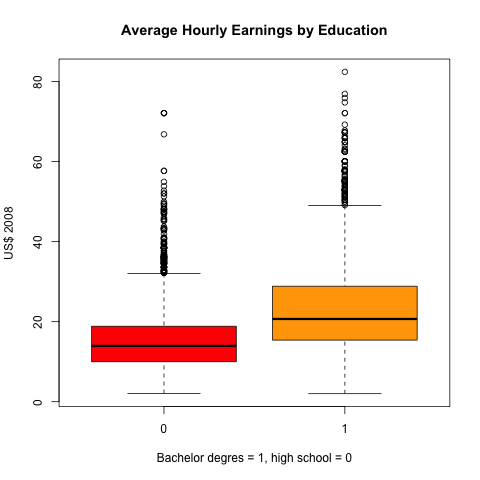
\includegraphics[width=.9\linewidth]{figure/boxplot.png}
\end{center}

\subsection*{Question (e)}
\label{sec:org9fb4fa2}

We repeat the steps in (d) by replacing the 2008 data with the 1992
data and using the inflation-adjusted average hourly earnings.

\begin{verbatim}
# select data in 2008
cps92 <- subset(cpsdat, year == 1992)

# calculate means
ahe.educ.92 <- aggregate(ahe.adj ~ bachelor, FUN = mean, data = cps92)

# select ahe and filter by bachelor
ahe.high.92 <- with(cps92, ahe.adj[bachelor == 0])
ahe.bach.92 <- with(cps92, ahe.adj[bachelor == 1])

# construct confindence interval
t.ahe.high.92 <- t.test(ahe.high.92)
t.ahe.bach.92 <- t.test(ahe.bach.92)
t.ahe.gap.92 <- t.test(ahe.bach.92, ahe.high.92)
\end{verbatim}

\begin{itemize}
\item The mean of the average hourly earnings of high school graduates in
1992 is equivalent to \texttt{15.31} the
2008 dollars with the 95\%
confidence interval (\texttt{15.11},
\texttt{15.52}).
\item The mean of the average hourly earnings of college graduates in 1992
is \texttt{21.78} in the 2008 dollars with
the 95\% confidence interval
(\texttt{21.45},
\texttt{22.12}).
\item The 95\% confidence interval of the gap in earnings between the two
groups is
(\texttt{6.08},
\texttt{6.86}).
\end{itemize}
\end{document}